\chapter{PROSPECT}

The scientific community's understanding of neutrinos has come a long way from Pauli's initial proposition of its existence in 1930. 
Though three active neutrino flavors and their behaviors are understood and well included in the Standard Model of particle physics, recent anomalies in reactor neutrino experiment results hint at the possibility of new physics. 
The discovery of an eV-scale sterile neutrino would have wide ranging impacts on the field of neutrino physics and future experiments.

The Precision Reactor Oscillation and Spectrum Experiment (PROSPECT) is designed to address the reactor antineutrino anomaly by performing a reactor-model independent search for short-baseline $\bar{\nu_{e}}$ oscillations and making a high precise measurement of the $^{235}$U $\bar{\nu_{e}}$ energy spectrum at a highly-enriched uranium (HEU) research reactor.
Located at the High Flux Isotope Reactor (HFIR) at Oak Ridge National Laboratory (ORNL) in Tennessee PROSPECT also demonstrates successful application of techniques for antineutrino detection at the surface with little overburden. 
PROSPECT collected data from May to December of 2018 and the first oscillation and spectrum results, with 33 and 40.3 live-days of reactor on time respectively, can be found in Ref.\cite{PhysRevLett.121.251802,Ashenfelter:2018jrx}.

\section{HFIR}

\begin{figure}
	\centering
	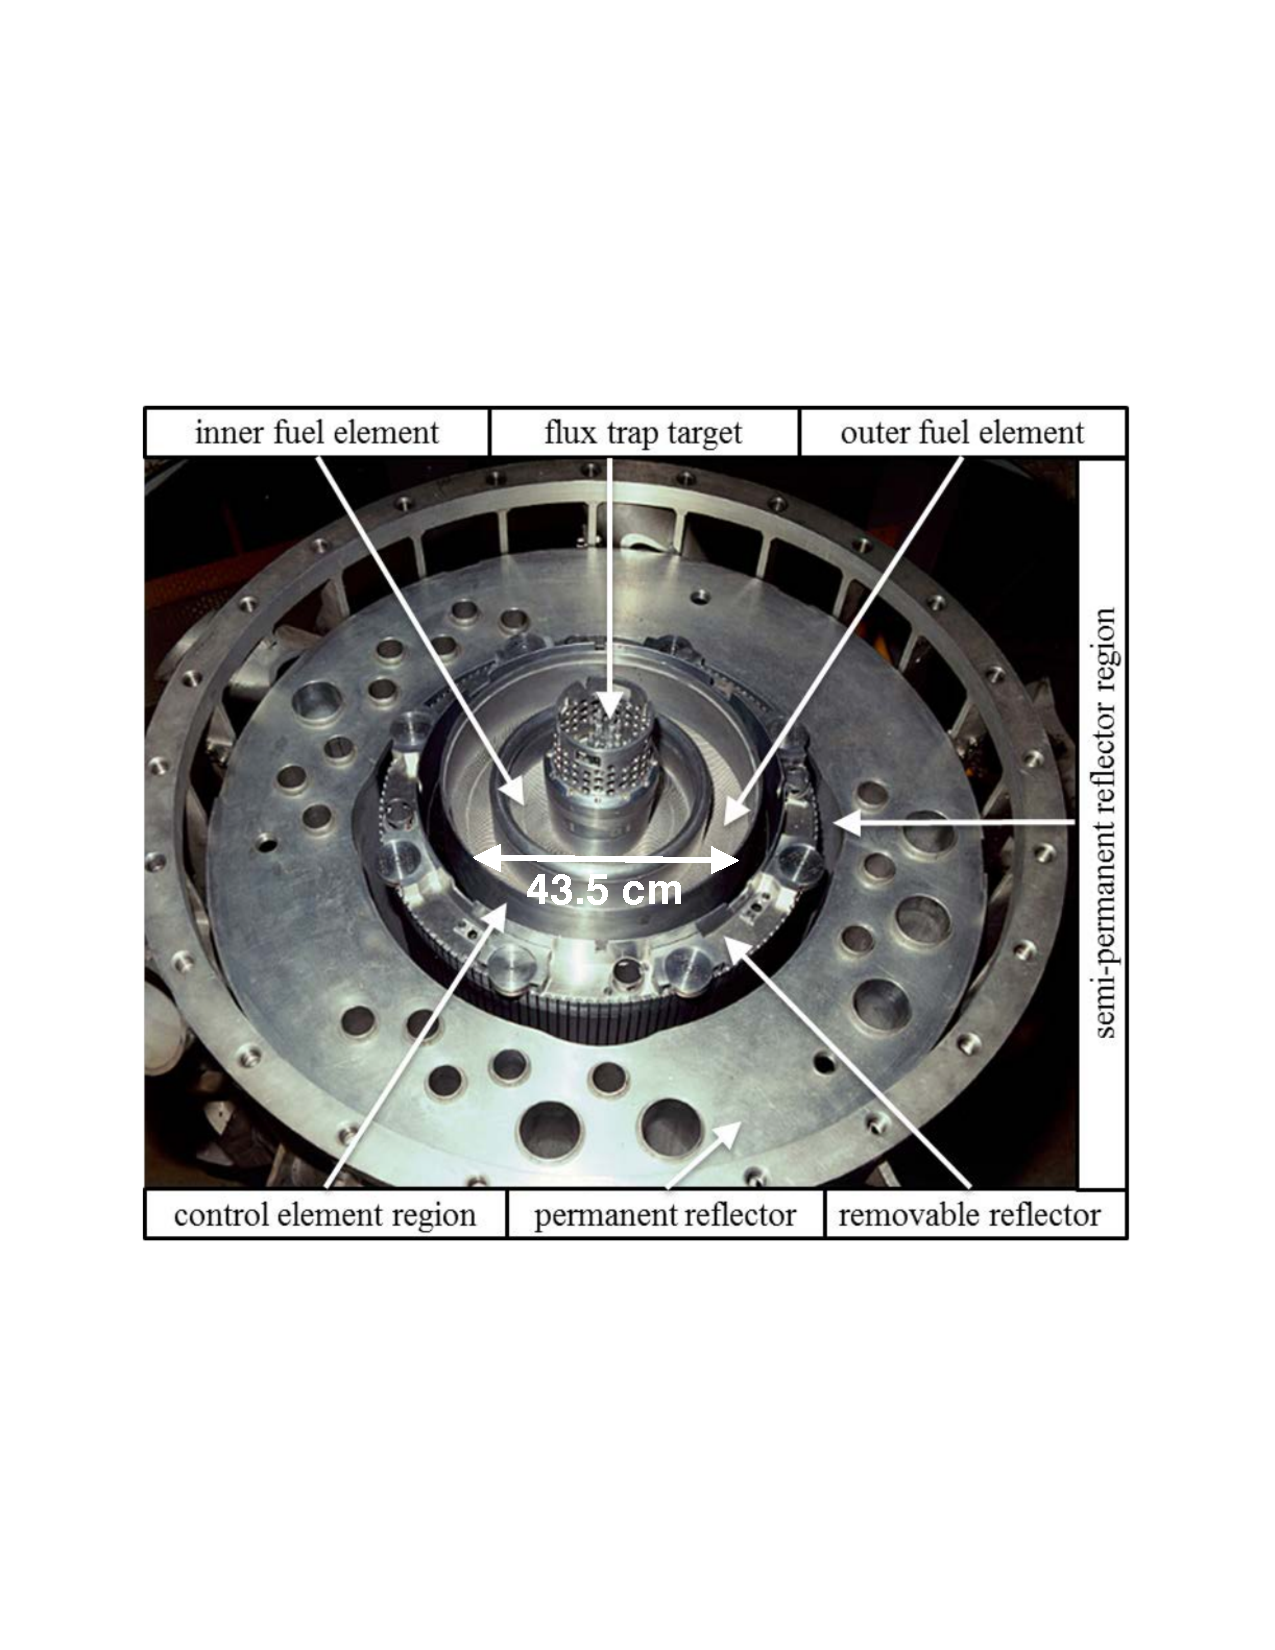
\includegraphics[width=0.7\linewidth]{tex/4-prospect-images/HFIRCore}
	\caption[]{\cite{HFIRTech}}
	\label{fig:hfircore}
\end{figure}



\section{Design}

\section{Detecting Inverse Beta Decays}

\section{From Signal to Result}


